\chapter{対話型遺伝的アルゴリズム}
本章では,本システムで使用した対話型遺伝的アルゴリズムを概説する.
\section{遺伝的アルゴリズム}
遺伝的アルゴリズム(Genetic Algorithm;GA)は、生物が環境に適応し進化する過程を模倣した最適解探索アルゴリズムである。問題に対する解を個体の染色体とし、解の構成要素を遺伝子として表現する。個体の評価、交叉、突然変異によって複数の個体を進化させ,環境に適応できる個体を見つけることで最適解を導く。基本アルゴリズムのフローチャートを図3.1に示す。

\subsection{染色体}
生物の各個体の形質や遺伝情報は、遺伝子によって決定される。
GAでは、解に関する情報を示す値を遺伝子と呼び、遺伝子を配列にしたものを染色体と呼ぶ。
遺伝子が配置される位置を表す番号を遺伝子座、配列として表現される遺伝子の構成を遺伝子型、遺伝子から発現した形質を表現型と呼ぶ。

\begin{figure}[htbp]
	\begin{center}
		\includegraphics[scale=0.3]{image/flowchart.pdf}
		\caption{遺伝的アルゴリズムのフローチャート}
	\end{center}
\end{figure}

\subsection{個体の評価}
染色体をもとに構成された表現型は個体と呼ばれ、各個体の解としての良さが評価される。評価結果を表す数値を適応度、適応度を求める関数を適応度関数と呼ぶ。

\subsection{次世代生成}
GAでは、よりよい個体群を生成するために、個体群内のすべての個体の適応度を算出し、算出された適応度をもとに次世代の個体群を生成する。次世代個体は、親個体選択によって選択された2つの個体を親とし、交叉と突然変異によって生成される。

\subsubsection{親個体選択}
親個体の選択手法には、ルーレット選択、ランキング選択、トーナメント選択等が存在する。ルーレット選択は、各個体が持つ適応度の比を確率にして選択する手法である。図3.2に示すような円盤全体の面積に対する各個体の面積の割合が、親個体の選択確率となる。ランキング選択は、個体群内における順位に応じて選択確率を決定し、親個体を選択する手法である。トーナメント選択は、個体群内からランダムに選択したいくつかの個体のうち、最も適応度が高い個体を親個体として選択する手法である。

\subsection{交叉}
交叉とは、選択された個体同士で遺伝子を交換する手法である。個体同士を交叉させることで、お互いの形質を持った次世代の個体を生成する。交叉手法には、一点交叉、二点交差、n点交叉、一様交叉等が存在する。一点交叉とは、図3.3(1)のように染色体における遺伝子間の位置をランダムに1箇所選び、前後の遺伝子列を交換する手法である。二点交差は、図3.3(2)のように染色体における遺伝子間の位置をランダムに2箇所選び、1つ目の点と2つ目の点で2回の遺伝子列を交換する手法である。n点交叉は、2点交叉と同様の手順でn回の遺伝子列を交換する手法である。一様交叉は、図3.3(3)のように子個体に受け継ぐ遺伝子を遺伝子座ごとに決定し、遺伝子を交換する手法である。

\begin{figure}[htbp]
	\begin{center}
		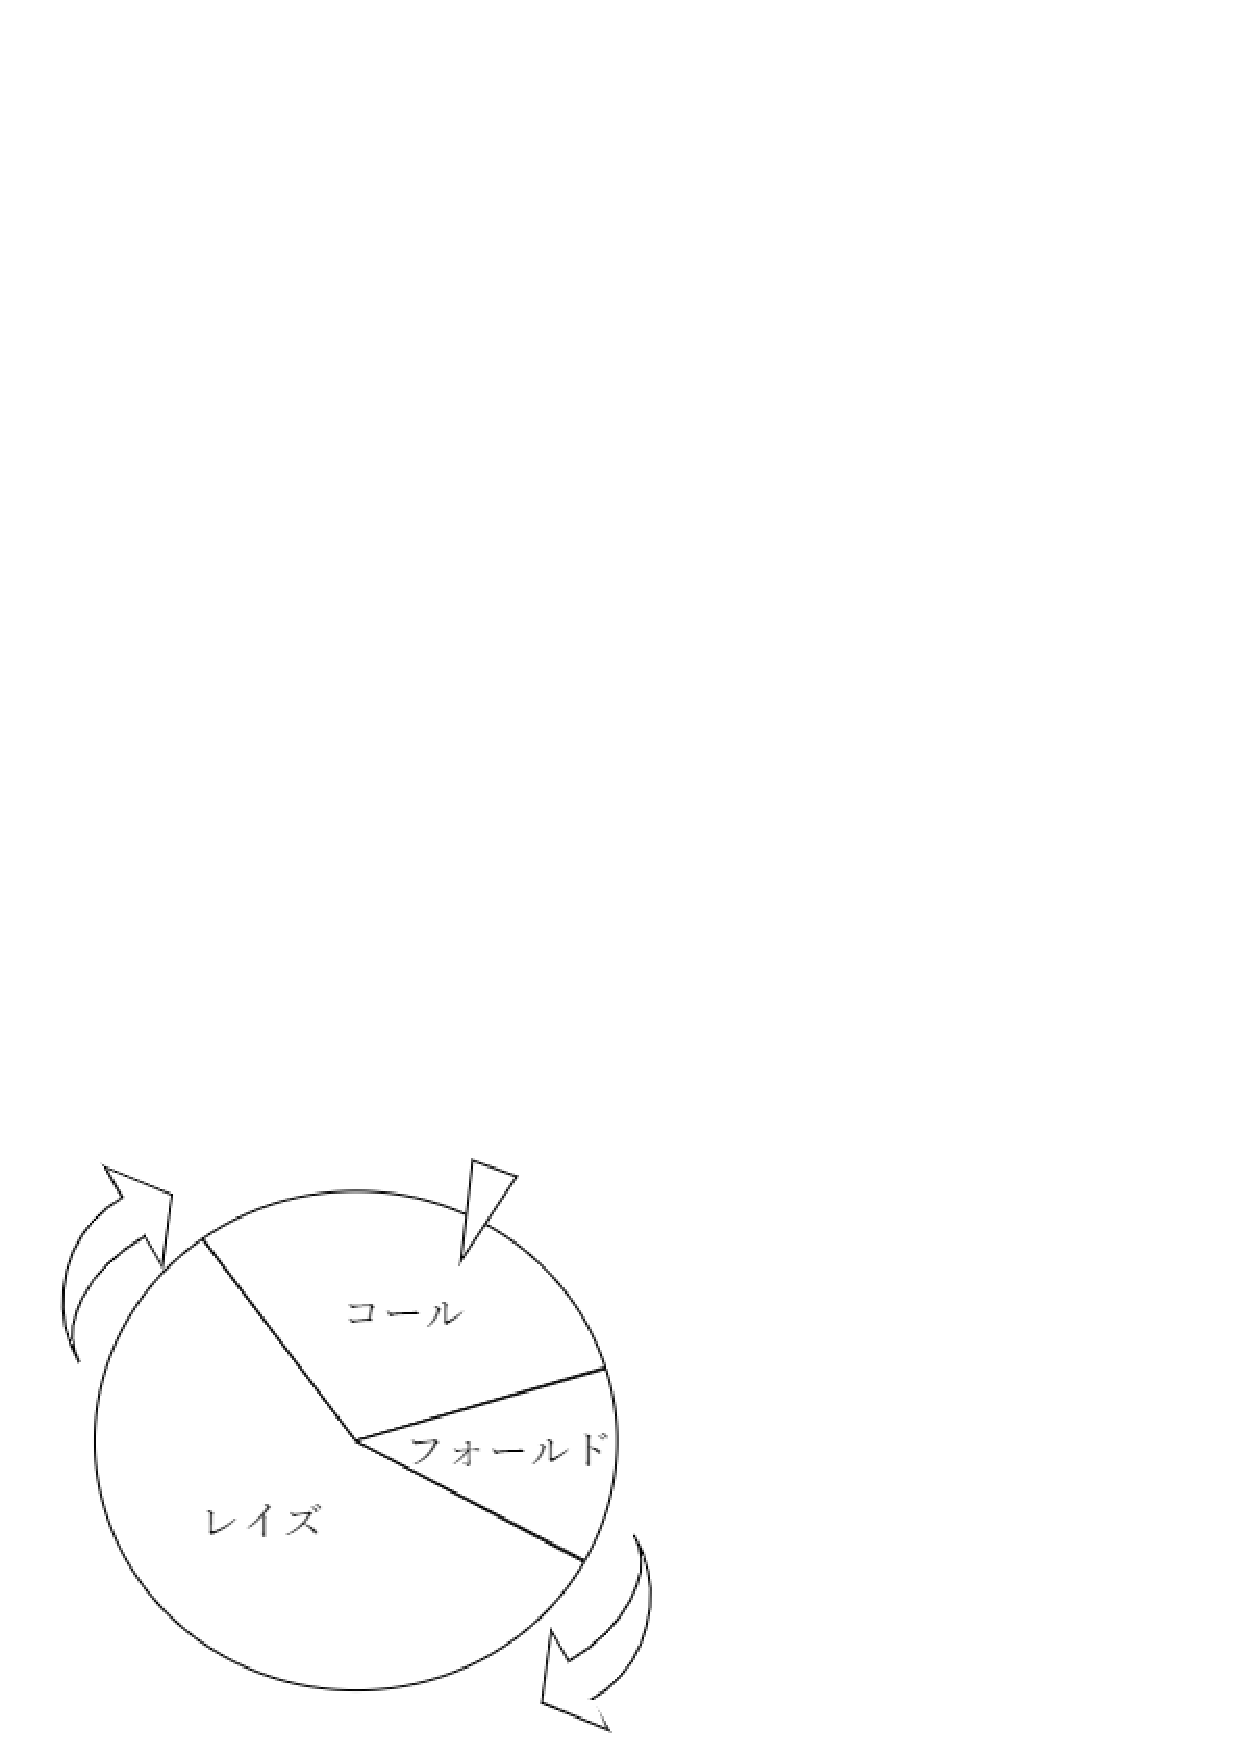
\includegraphics[scale=0.2]{image/roulette.pdf}
		\caption{ルーレット選択}
	\end{center}
\end{figure}

\begin{figure}[htbp]
	\begin{center}
		\includegraphics[scale=0.25]{image/onepointCrossover.pdf}
    \vskip\baselineskip
    \includegraphics[scale=0.25]{image/twopointCrossover.pdf}
    \vskip\baselineskip
    \includegraphics[scale=0.25]{image/uniformCrossover.pdf}
    \vskip\baselineskip
		\caption{交叉}
	\end{center}
\end{figure}

\subsection{突然変異}
突然変異とは、交叉によって生成された個体の遺伝子を、設定した任意の確率に基づいて変異させることである。突然変異することで局所最適解への収束を防ぐことができるが、親個体から受け継いだ形質を失う可能性があるため、適切な確率設定が必要となる。
\subsection{進化戦略}
親個体同士の組み合わせや交叉手法によって、親の形質が引き継がれず適応度が悪化する可能性がある。優良個体を失うのを防ぐために、最優良個体を次世代に残すエリート保存戦略と呼ばれる戦略がある。

\section{対話型遺伝的アルゴリズム}
対話型遺伝的アルゴリズム(IGA; Interactive Genetic Algorithm )は、GAの一種であり、人間が持つ感性を評価関数とし、最適解を求める手法である。適応度関数の設定が困難であり、人間の好みに基づいた生成に対して用いられる。